% !TEX root = Main.tex

In this section we introduce important lemmas, definitions and tricks we will use throughout. This is intended as a quick lookup location containing most relevant lemmas/definitions.

We start with one of the most important definitions to remember, as this will be the basis of our reachability algorithm.

\begin{definition} \label{DefinitionGoodOverapproximation}
Let \(\vectSet{X} \subseteq \vectSet{L} \subseteq \N^{d}\) be sets with \(\vectSet{L}=\vect{b}+\N(\vectSet{F})\) being linear. Then \(\vectSet{L}\) is a \emph{nice overapproximation} of \(\vectSet{X}\) (written \(\vectSet{X} \HybridizationRelation \vectSet{L}\)) if for every \(\vect{x} \in \vectSet{L}\) and every \(\vect{w} \in \N_{\geq 1}(\vectSet{F})\), there exists \(N \in \N\) such that \(\vect{x}+\N_{\geq N}\vect{w} \subseteq \vectSet{X}\). 

Observe the \(\N_{\geq 1}(\vectSet{F})\) instead of \(\N(\vectSet{F})\), which is crucial.

This definition applies to relations \(\vectSet{X}, \vectSet{L} \subseteq \N^{d_1} \times \N^{d_2}\) by viewing them as sets \(\vectSet{X}, \vectSet{L} \subseteq \N^{d_1+d_2}\).
\end{definition}

I.e.\ a linear overapproximation \(\vectSet{L}\) of a relation \(\vectSet{X}\) is nice if starting at any point \(\vect{x} \in \vectSet{L}\) and ``walking in an interior direction'' \(\vect{w}\) of \(\vectSet{L}\), eventually all the visited points are in \(\vectSet{X}\). Since this is a very central notion, let us carefully introduce an example and some properties.

Observe first of all that clearly every linear set \(\vectSet{L}\) is nicely overapproximated by itself. But a more interesting example is on the right of Figure \ref{FigureIntuitionSemilinearityAlgorithm}: While \(\vectSet{X}\) is non-semilinear, as long as \(\vect{w}\) is not ``vertical'', i.e.\ \(\N_{\geq 1}\) is indeed crucial, one can find an \(N\) as in Definition \ref{DefinitionGoodOverapproximation}. Observe also that there is no uniform \(N \in \N\) which works for every \(\vect{x}, \vect{w}\): Different \(\vect{x} \in \N^2\) can have a different ``distance'' from \(\vectSet{X}\).

\begin{figure}[h!]
\begin{minipage}{4.5cm}
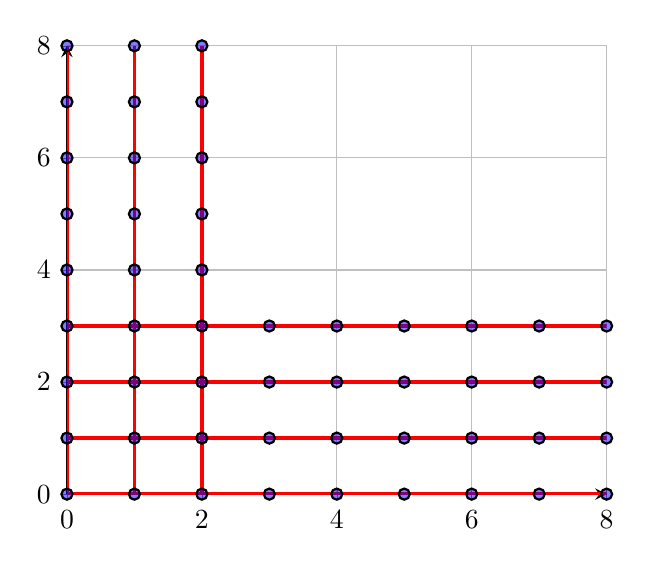
\begin{tikzpicture}
\begin{axis}[
    axis lines = left,
    xlabel = { },
    ylabel = { },
    xmin=0, xmax=8,
    ymin=0, ymax=8,
    xtick={0,2,4,6,8},
    ytick={0,2,4,6,8},
    ymajorgrids=true,
    xmajorgrids=true,
    thick,
    smooth,
    no markers,
]

\addplot[
    fill=blue,
    fill opacity=0.5,
    only marks,
    ]
    coordinates {
    (0,0)(0,1)(0,2)(0,3)(0,4)(0,5)(0,6)(0,7)(0,8)(1,0)(2,0)(3,0)(4,0)(5,0)(6,0)(7,0)(8,0)(1,1)(1,2)(1,3)(1,4)(1,5)(1,6)(1,7)(1,8)(2,1)(2,2)(2,3)(2,4)(2,5)(2,6)(2,7)(2,8)(3,1)(3,2)(3,3)(4,1)(4,2)(4,3)(5,1)(5,2)(5,3)(6,1)(6,2)(6,3)(7,1)(7,2)(7,3)(8,1)(8,2)(8,3)
    };
    
%\addplot[
%    fill=green,
%    fill opacity=0.7,
%    only marks,
%    ]
%    coordinates {
%    (3,4)(3,5)(3,6)(3,7)(3,8)(4,4)(4,5)(4,6)(4,7)(4,8)(5,4)(5,5)(5,6)(5,7)(5,8)(6,4)(6,5)(6,6)(6,7)(6,8)(7,4)(7,5)(7,6)(7,7)(7,8)(8,4)(8,5)(8,6)(8,7)(8,8)
%    };
    
\addplot[
   draw=red,
   no marks,
   very thick,
   ]
   coordinates {
   (0,0)(0,8)
   };
   
\addplot[
   draw=red,
   no marks,
   very thick,
   ]
   coordinates {
   (1,0)(1,8)
   };
   
\addplot[
   draw=red,
   no marks,
   very thick,
   ]
   coordinates {
   (2,0)(2,8)
   };
   
\addplot[
   draw=red,
   no marks,
   very thick,
   ]
   coordinates {
   (0,0)(8,0)
   };
   
\addplot[
   draw=red,
   no marks,
   very thick,
   ]
   coordinates {
   (0,1)(8,1)
   };
   
\addplot[
   draw=red,
   no marks,
   very thick,
   ]
   coordinates {
   (0,2)(8,2)
   };
   
\addplot[
   draw=red,
   no marks,
   very thick,
   ]
   coordinates {
   (0,3)(8,3)
   };

\end{axis}
\end{tikzpicture}
\end{minipage}%
\begin{minipage}{4.5cm}
\begin{tikzpicture}
\begin{axis}[
    axis lines = left,
    xlabel = { },
    ylabel = { },
    xmin=0, xmax=4,
    ymin=0, ymax=16,
    xtick={0,1,2,3,4},
    %ytick={0,1,2,3,4,5,6,7,8,9,10,11,12,13,14,15,16},
    ytick={0,4,9,16},
    ymajorgrids=true,
    xmajorgrids=true,
    thick,
    smooth,
    no markers,
]
    
\addplot[
    fill=blue,
    fill opacity=0.5,
    only marks,
    ]
    coordinates {
    (0,0)(1,0)(1,1)(2,0)(2,1)(2,2)(2,3)(2,4)(3,0)(3,1)(3,2)(3,3)(3,4)(3,5)(3,6)(3,7)(3,8)(3,9)(4,0)(4,1)(4,2)(4,3)(4,4)(4,5)(4,6)(4,7)(4,8)(4,9)(4,10)(4,11)(4,12)(4,13)(4,14)(4,15)(4,16)
    };
    
\addplot[
    name path=A,
    domain=0:4,
    color=red,
]
{x^2};

\end{axis}
\end{tikzpicture}
\end{minipage}%

\caption{\textit{Left}: Illustration of \(\dim(\vectSet{L} \setminus (\vect{p}+\vectSet{L}))<\dim(\vectSet{L})\) with \(\vectSet{L}=\N^2\) and \(\vect{x}=(3,4)\). The dimension drops from 2 to 1, since the set is now coverable by finitely many lines.  \newline
\textit{Right}: \(\vectSet{X}=\{(x,y)\in \N^2 \mid y \leq x^2\}\) has the nice overapproximation \(\N^2\).}\label{FigureIntuitionSemilinearityAlgorithm}
\end{figure}

Some more in-depth understanding of nice overapproximations can be gained by considering closure properties:

\begin{restatable}{lemma}{LemmaShiftGoodOverapproximation} \label{LemmaShiftGoodOverapproximation}
Let \(\vectSet{X} \HybridizationRelation \vectSet{L}\) and let \(\vectSet{L}'\) a linear set s.t. \(\vectSet{L} \cap \vectSet{L}'\) is non-degenerate and remains linear. Then \(\vectSet{X} \cap \vectSet{L}' \HybridizationRelation \vectSet{L} \cap \vectSet{L}'\).

Let \(\vectSet{X}_{12} \HybridizationRelation \vectSet{L}_{12} \subseteq \N^{d_1} \times \N^{d_2}\) and \(\vectSet{X}_{23} \HybridizationRelation \vectSet{L}_{23}\subseteq \N^{d_2} \times \N^{d_3}\). Assume that \(\pi_{in}(\vectSet{L}_{23}) \cap \pi_{out}(\vectSet{L}_{12})\) is non-degenerate, where \(\pi_{in} \colon \N^{d_2} \times \N^{d_3} \to \N^{d_2}\) and \(\pi_{out} \colon \N^{d_1} \times \N^{d_2} \to \N^{d_2}\) are the projections to in- and output. Then \(\vectSet{X}_{12} \circ \vectSet{X}_{23} \HybridizationRelation \vectSet{L}_{12} \circ \vectSet{L}_{23}\).
\end{restatable}

\begin{proof}[Proof sketch]
Observe that the definition of nice overapproximation makes a claim about every point \(\vect{x}\in \vectSet{L}\) and every \(\vect{w} \in \N_{\geq 1}(\vectSet{F})\), hence decreasing \(\vectSet{L}\) and decreasing the set \(\N_{\geq 1}(\vectSet{F})\) of possible \(\vect{w}\)'s preserves the property. Hence the main part of the proof is to check that \(\N_{\geq 1}(\vectSet{F})\) decreases through the intersection/composition. The formal proof is in the appendix, but let us observe here that if we for example intersect \(\N^2 \cap \{0\} \times \N\), then \(\N_{\geq 1}(\{(1,0),(0,1)\}) \not \subseteq \N_{\geq 1}(\{(0,1)\})\): We would exactly get the vertical direction \(\vect{w}\) as before. Therefore the non-degenerate intersection is crucial.
\end{proof}

In order for nice overapproximations to be useful, we need an algorithm which given \(\vectSet{X}\in \RelationClass\), splits it into finitely many parts with a nice overapproximation each.

\begin{definition} \label{DefinitionApproximable}
Let \(\RelationClass\) be a class of relations. Then \(\RelationClass\) is \emph{approximable} in \(\mathfrak{F}_{\alpha}\) if there is an algorithm with running time in \(\mathfrak{F}_{\alpha}\) which given \(\vectSet{X} \in \RelationClass\), outputs finitely many \(\vectSet{X}_1, \dots, \vectSet{X}_k \in \RelationClass\), linear relations \(\vectSet{L}_1, \dots, \vectSet{L}_k\) and a function \(g \in \mathfrak{F}_{\alpha}\) s.t. 
\begin{enumerate}
\item \(\vectSet{X}=\bigcup_{j=1}^k \vectSet{X}_j\),
\item If \(\vectSet{X}\) is monotone, then also the \(\vectSet{X}_j\).
\item \(\forall\ 1 \leq i \leq k\) we have \(\vectSet{X}_j \HybridizationRelation \vectSet{L}_j\) and 
\item \(N\) in Definition \ref{DefinitionGoodOverapproximation} fulfills 

\(\size(N) \leq g(\size(\vectSet{X}_j)+\size(\vect{x})+\size(\vect{w}))\).
\end{enumerate}
\end{definition}

We will later give such an algorithm for a large class of eVASS, in particular VASS, \ConsideredModel, etc.

Let us illustrate one \emph{main} trick in our toolbox: On the left of Figure \ref{FigureIntuitionSemilinearityAlgorithm}, we illustrate an important lemma we use often:

\begin{lemma}[\cite{Leroux13}, Corollary D.2] \label{LemmaDimensionDecreaseShiftedL}
Let \(\vectSet{L}=\vect{b}+\N(\vectSet{F})\) be linear, and \(\vect{p} \in \N(\vectSet{F})\). Then \(\dim(\vectSet{L} \setminus \vect{p}+\vectSet{L})<\dim(\vectSet{L})\).
\end{lemma}

Both Lemma \ref{LemmaShiftGoodOverapproximation} and Lemma \ref{LemmaDimensionDecreaseShiftedL} can be used for recursion in algorithms: By Lemma \ref{LemmaShiftGoodOverapproximation}, problems only occur if the intersection has lower dimension, and by Lemma \ref{LemmaDimensionDecreaseShiftedL}, it is sufficient to understand a set \emph{asymptotically}, as we can deal with the rest via an appropriate recursion.

Finally, since we will often have to deal with projections, which can be slightly annoying, we use the following:

\begin{lemma} \label{LemmaNiceOverapproximationProjection}
Let \(\vectSet{X} \HybridizationRelation \vectSet{L}\), and \(\pi\) a proj.. Then \(\pi(\vectSet{X}) \HybridizationRelation \pi(\vectSet{L})\).
\end{lemma}

\begin{proof}
Immediate from the definition.
\end{proof}



















































